%!TEX root = main.tex

The \textbf{syntax} correspond to an arrangement to form correct sentences. A \textbf{formal grammar} is the set of rules which define the syntax. The \textbf{syntactic analysis} is the application of formal rules to filter grammatical and ungrammatical sentences. There is three fundamental concepts in formal grammar.

\begin{itemize}
	\item \textbf{Constituency}: a group of words may behave as a single unit. For example, nominal sentences. There is two clues of words that are grouped togheter: the first one is the context (before a verb for example) and the second is that we can move the group of word in different places of the sentence (preposed/postposed constructions);
	\item \textbf{Grammatical relations}: formalization of ideas from traditional grammar (Subject/Object);
	\item \textbf{Subcategorization and dependency relations}: Some types of relations between word and phrases (for example transitive verbs like \textit{find}).
\end{itemize}

\subsection{Context Free Grammar}

A CFG consists of a set of rules and a lexicon of words and symbols.
\begin{itemize}
	\item $N$ a set of non-termina symbols;
	\item $\sum$ a set of terminal symbols;
	\item $R$ a set of rules of the form $A \rightarrow \beta$;
	\begin{itemize}
		\item $A$ is non-terminal;
		\item $\beta$ is a string of symbols: $(N \cup \sum)^*$.
	\end{itemize}
	\item $S$ a start symbol.
\end{itemize}

A CFG define a formal language. The term generative grammar underlines the fact that in this approach a language is defined by a set of possible sentences generated by the grammar.

\subsection{Some grammar rules and syntactic structures}

\subsubsection{Agreement problem}

To handle the particular cases (for example a verb which take \textit{s} at the third singular form), we need to add rules on the grammar. The consequence is a increase of the size of the grammar. A solution is to use a constraint-based formalism to take into accont fine-grained information about number and person agreement, subcategorization and even semantic categories.

\begin{figure}[htp]
	\centering
	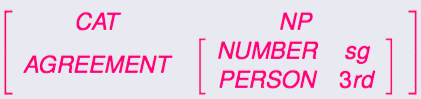
\includegraphics[scale=0.4]{images/41_matrix.png}
 	\caption{Feature structure.}
\end{figure}

\subsubsection{Subcategorization}

All verbs are not compatible with all kind of constituents. The solution is to have different catagories of words (for example, transitive verb and instransitive verb).

\subsubsection{Treebank}

\begin{figure}[htp]
	\centering
	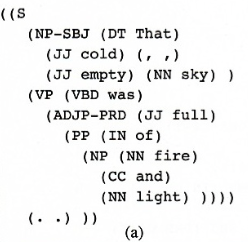
\includegraphics[scale=0.4]{images/42_treebank.png}
 	\caption{Brown treebank.}
\end{figure}

\subsection{Dependency Grammars}

In dependency grammars, constituents and phrase structure rules do not play any fundamental role. Instead, the syntactic structure of a sentence is described purely in terms of words and binary semantic or syntactic relations between these words (called lexical dependencies). Dependency grammars use dependency relationships between lexicon elements. The nature of the relationship can be morphologic, syntaxic or semantic. The main advantage is to handle languages with free word order (Czech, Latin).